% \hiddensubsection{Introduction}
\label{sec:intro}
With the intention of making robotics education more accessible, The Manipulator for Educational Institutions with Open Source Integrated Systems (MEIOSIS) intends to provide high school educators and robot enthusiasts with a low cost manipulator. The system should be usable by novice students. It should also be modifiable to create a sustainably increased understanding of robotics. While MEIOSIS may not fully emulate industrial manipulators, it aims to provide more students with access to robotics education. \\
\begin{figure}[htp]
  \centering
  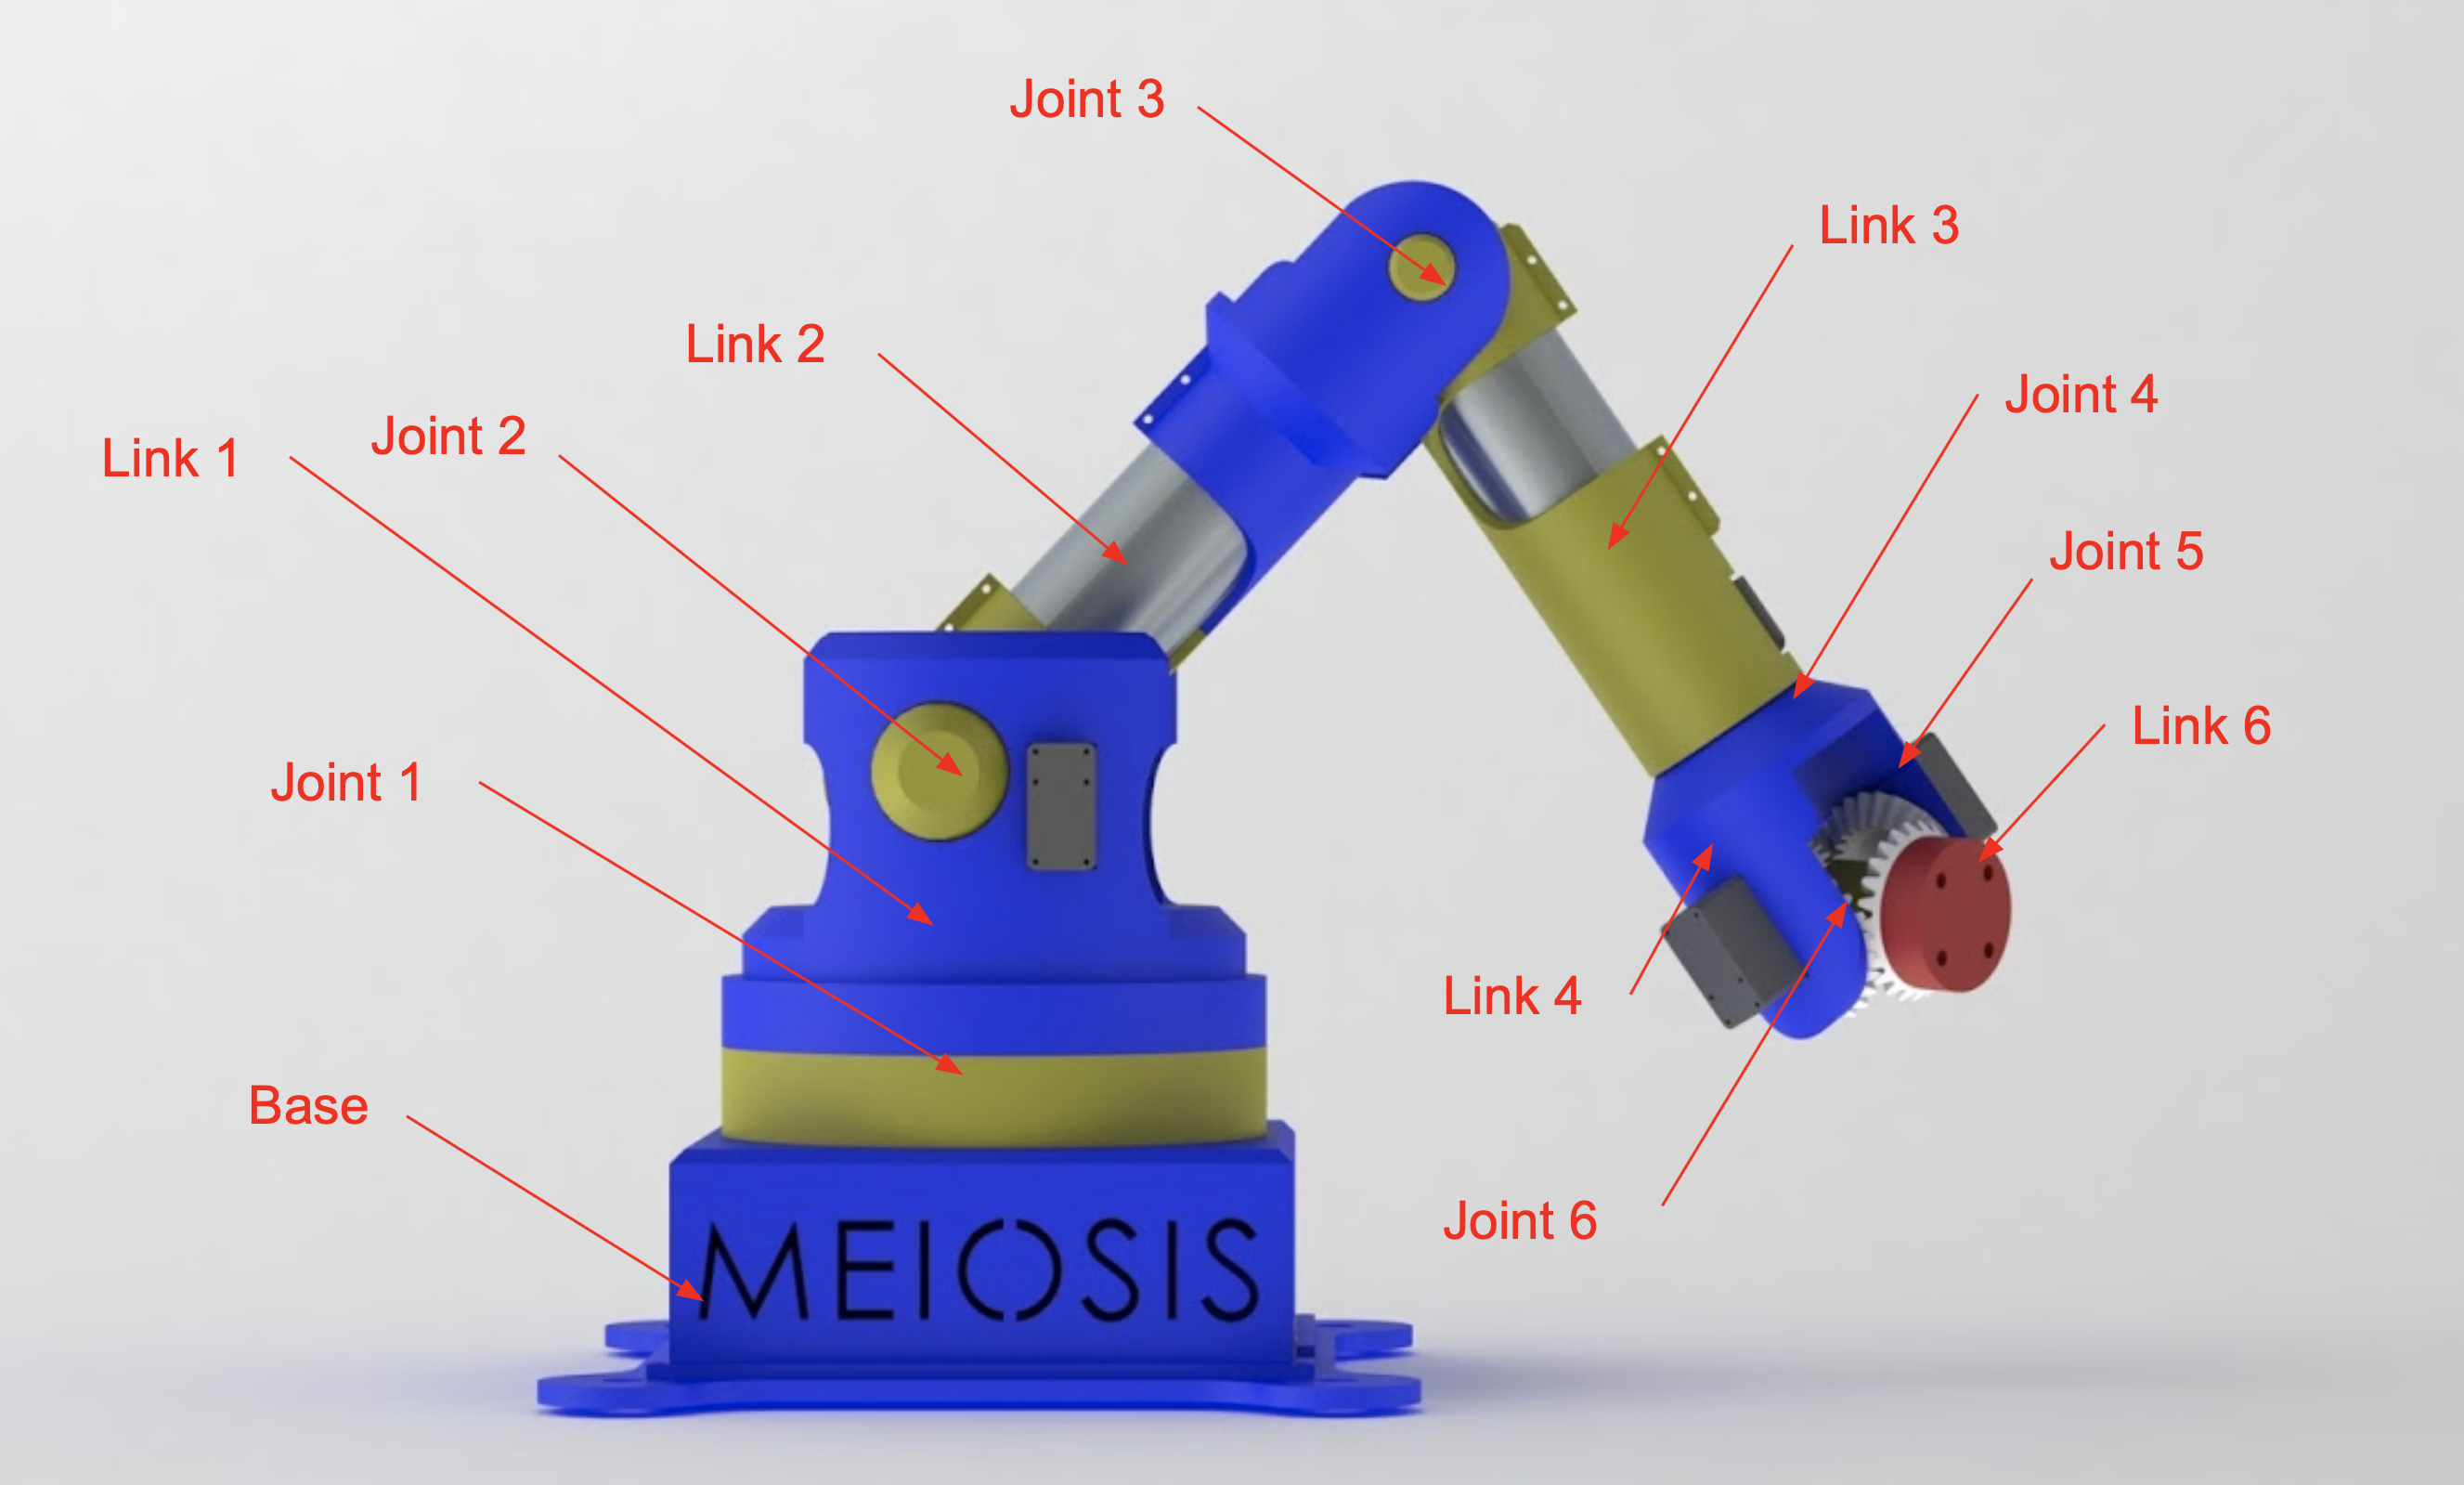
\includegraphics[frame,width=.75\textwidth]{model}
  \caption{Overview of Physical System}
  \label{fig:model}
\end{figure}
\newline
The design seen in \emph{Figure \ref{fig:model}} is based on our conceptual design. It features four links and six joints for rotation and will be referenced throughout this document. The base of the manipulator and end-effector can also be seen in the figure.
\hiddensubsection{Design Requirements}
The specifications of the system are strictly based on the requirements defined previously. The requirements are divided into two primary categories, hardware and software.
\vspace{-\baselineskip}
\hiddensubsection{Hardware}
The following requirements and specifications are hardware specific and dictate the physical constaints the system must adhere to.
\vspace{-\baselineskip}
\subsubsection{The system shall cost the end-user no more than \$1000.}
\begin{enumerate}
  \item \textit{The cost for the MEIOSIS team to develop the manipulator shall cost no more than \$800.}
\end{enumerate}

\subsubsection{The system shall be fully dexterous without being kinematically redundant.}
\begin{enumerate}
\item \textit{The system shall consist of six rotational joints connected by four links. The last three joints will create a spherical wrist.}
\end{enumerate}
As defined \cite{robo}, “A manipulator having more than six DOF is referred to as a kinematically redundant manipulator (5).” A manipulator with less than six degrees of freedom will not be fully dexterous within it's workspace. \emph{Figure \ref{fig:zero}} (see subsection \ref{sec:zero}, p. \pageref{fig:zero}) shows a six degree-of-freedom rotary manipulator with it's coordinate frames in zeroed positions. The joint and link locations are seen in \emph{Figure \ref{fig:model}} (see section \ref{sec:intro}, p. \pageref{sec:intro}).
\begin{enumerate}[resume]
\item \textit{The system shall have no link offsets.}
\end{enumerate}
Link offsets as seen in \emph{Figure \ref{fig:offset}} are commonly used to avoid singularities. However, having a link offset prevents the manipulator's dexterous workspace from being a complete hemispherical shell.

\begin{figure}[htp]
  \centering
  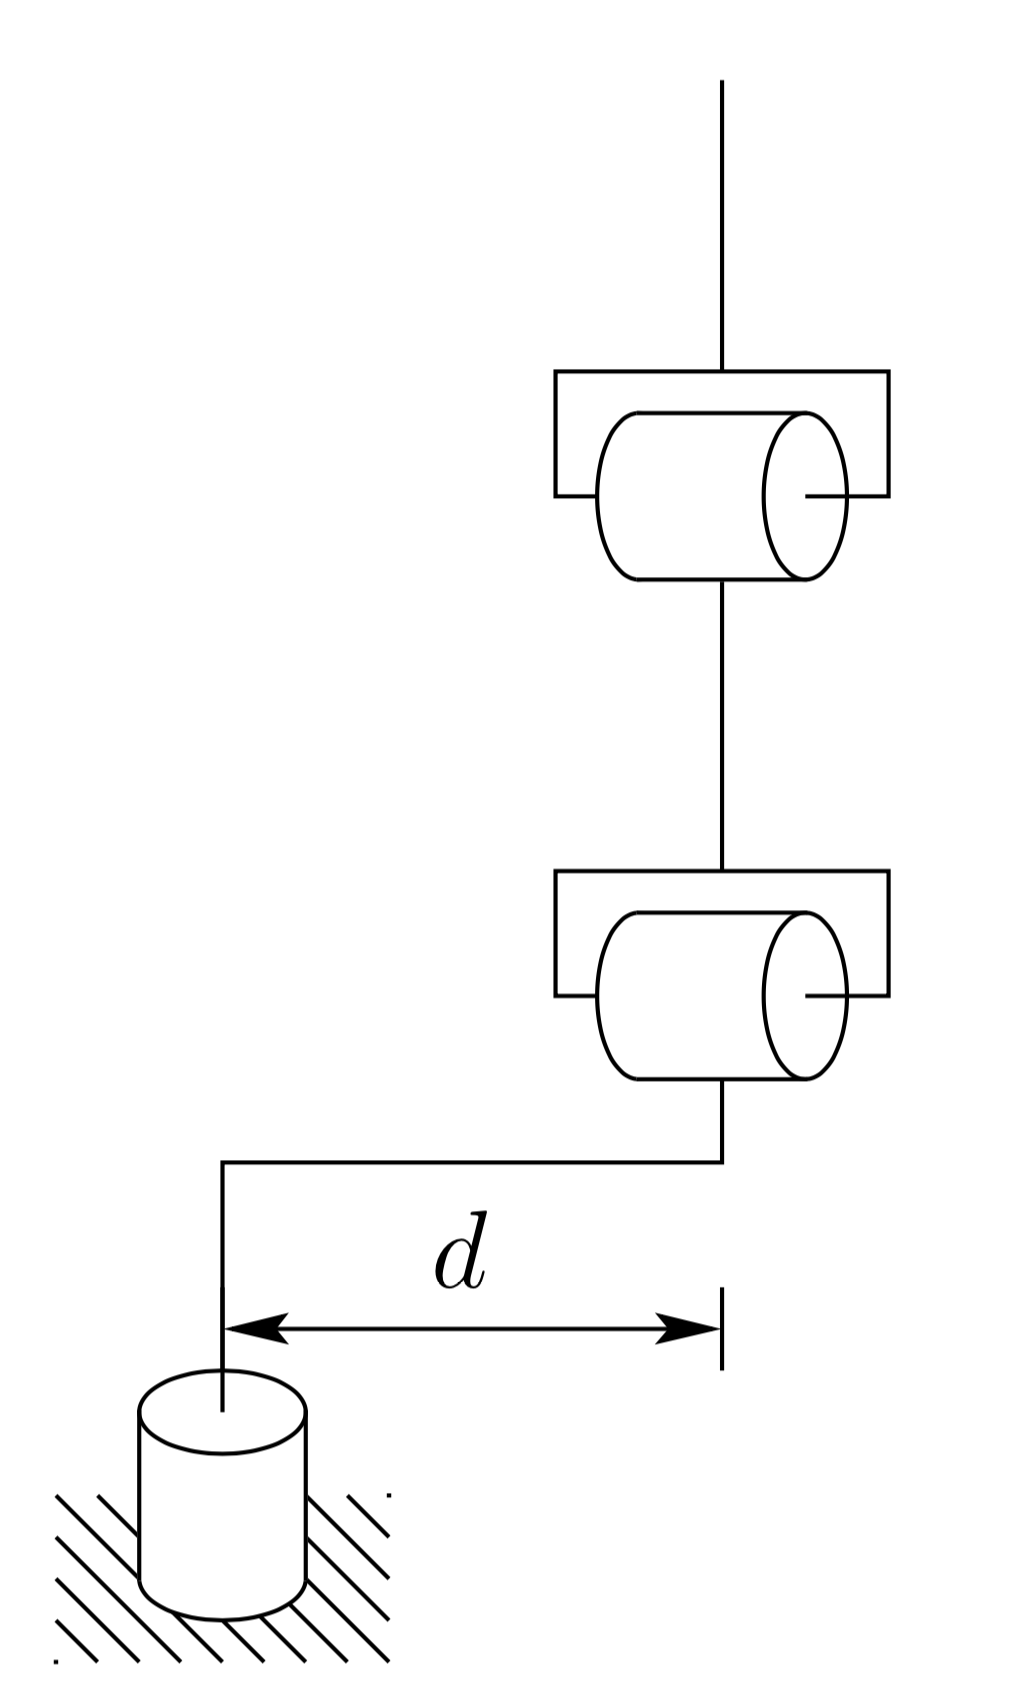
\includegraphics[width=.25\textwidth]{offset}
  \caption[Elbow Manipulator Configuration with Link Offset]{Elbow Manipulator Configuration with Link Offset \cite{robo}}
  \label{fig:offset}
\end{figure}
As shown in \emph{Figure \ref{fig:offset}}, the line directly above the first joint of the manipulator is offset such that the axes of the other joints are unable to become collinear with the base axis; this prevents singularity but causes a void in the detxterous workspace.
\subsubsection{The system end effector shall maintain a positional accuracy magnitude of \(\pm 1\) mm and an orientation accuracy of \(\pm 5^{\circ}\) eigen angle from the base frame.}
To ensure that the robot has educational value, the accuracy must be defined so that any desired positions and movements are achieved with sufficient accuracy.
\begin{enumerate}
  \item \textit{The system shall accommodate a process in which the end user can calibrate the end effector position and orientation to within 0.5 mm and 1 degree of the manipulator’s precision.}
\end{enumerate}
The addition of a calibration process allows the removal of any systematic errors, such as drift. The theoretical limit of the calibration process is the difference between the precision and accuracy metrics of the system.
\subsubsection{The system end effector shall maintain a pose repeatability magnitude between 0.1—1.5 mm for the position and \(\pm 4^{\circ}\) eigen angle from the base frame for the orientation.}
\begin{enumerate}
  \item \textit{Joint one and two of the system shall possess an angle error of no more than .025 degrees.}
\end{enumerate}
Being that joint one and two are the first two rotational elements in the system, their error will propagate the most to the end effector's position.
\begin{enumerate}[resume]
  \item \textit{Joint three of the system shall possess an angle error of no more than .03 degrees.}
\end{enumerate}
Since joint three is closer to the end effector it's error will not propagate as severely throughout the system.
\begin{enumerate}[resume]
  \item \textit{Joints four, five, and six shall possess an angle error of no more than .29 degrees.}
\end{enumerate}
The spherical wrist is the closest to the end effector's final position and therefore has the least error propagation.

\subsubsection{The system’s reachable workspace shall be a hemisphere with a radius of 300-700 mm.}
This workspace will provide enough movement to manipulate objects in order to perform basic tasks.
\begin{enumerate}
  \item \textit{The length of link one, two, three, four, and the wrist shall be 220.8 mm, 250 mm, 200 mm, 80 mm, and 52.5 mm respectively.}
\end{enumerate}
  This results in a total height of 220.8 mm with a total reach of 582.5 mm in the zeroed configuration as shown in the configuration represented in \emph{Figure \ref{fig:zero}}.

\subsubsection{The system’s dexterous workspace shall contain a hemispherical shell within the reachable workspace with a thickness of 280 mm.}\label{sec:zero}
This workspace will provide enough movement to manipulate objects in order to perform basic tasks. 280mm is slightly greater than the length of letter paper.
\begin{enumerate}
  \item \textit{The rotational limit of joint one, two, three, four, five, and six shall be \(\pm180^{\circ}\), \(-9.7^{\circ}\) to \(177.5^{\circ}\), \(-150.6^{\circ}\) to \(-19.3^{\circ}\), \(\pm180^{\circ}\), \(-180^{\circ}\) to \(-1.6^{\circ}\), and \(\pm180^{\circ}\) respectively.}
\end{enumerate}
The angles stated are with respect to the kinematic model shown in \emph{Figure \ref{fig:zero}}. To be fully dexterous within our 280 mm dexterous workspace the manipulator must have the joint angles specified above. The joint limitations were calculated by iteratively verifying the orientation about every point within the quarter hemisphere cross section seen in \emph{Figure \ref{fig:dex}} (see Appendix, p. \pageref{sec:app}).
  \begin{figure}[htp]
    \centering
    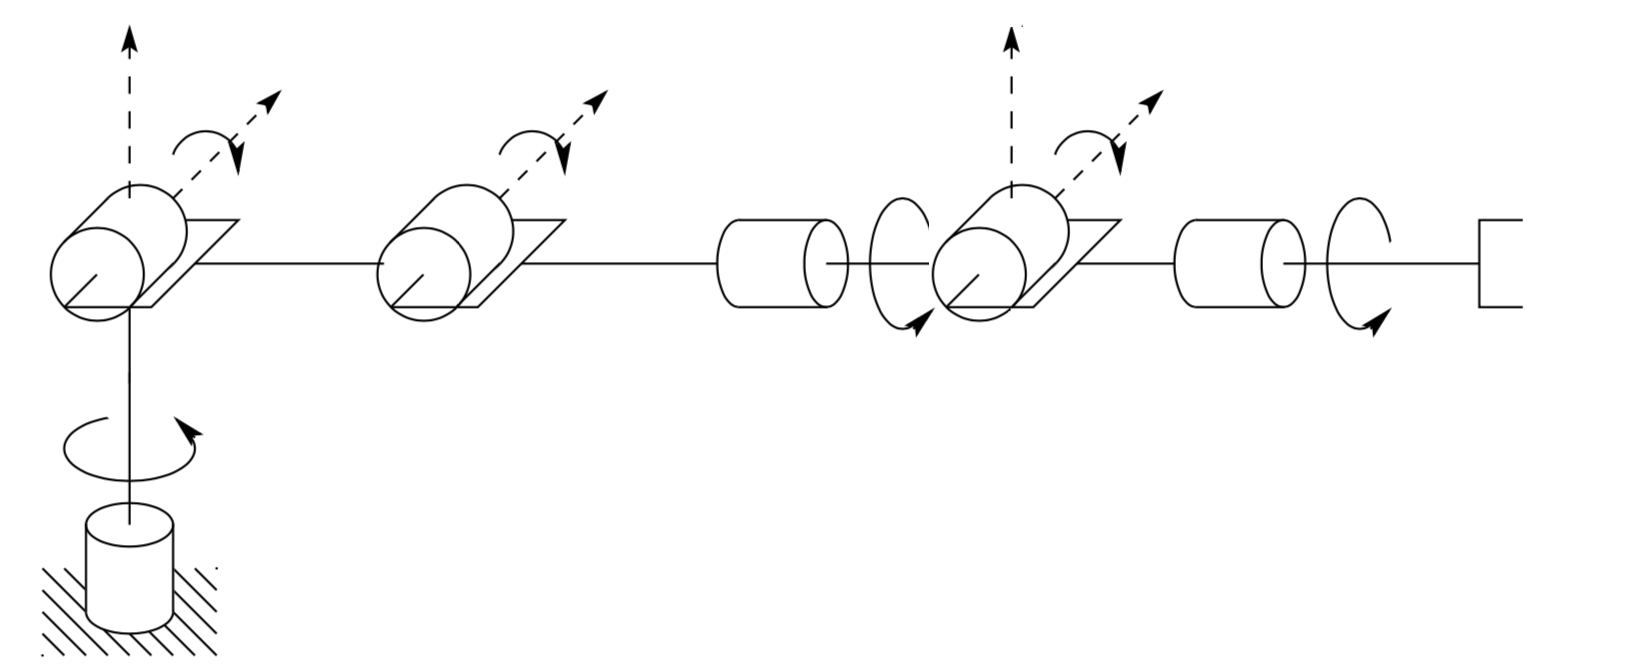
\includegraphics[width=.75\textwidth]{zero}
    \caption[Kinematic Model Representing Zeroed Configuration]{Kinematic Model Representing Zeroed Configuration \cite{robo}}
    \label{fig:zero}
  \end{figure}
\subsubsection{The system shall have a removable end effector capable of picking and placing a low-odor chisel tip Expo dry erase marker.}
This creates a robot capable of performing a variety of basic tasks, which enhances its educational value.
\begin{enumerate}
  \item \textit{The system shall use a parallel gripper that can close to 18mm.}
\end{enumerate}
The diameter of a low-odor chisel tip Expo dry erase marker is approximately 18 mm.
\begin{enumerate}[resume]
  \item \textit{The end effector shall attach to the manipulator using screws configured in a pattern that can accommodate a Dynamixel AX-12A servo.}
\end{enumerate}
It is expected that a majority of end effector styles will have to accommodate for a servo to facilitate actuation, therefore a pattern was chosen to standardize the mounting.


\subsubsection{The system shall be able to write with a low-odor chisel tip Expo dry erase marker.}
\begin{enumerate}
  \item \textit{The end effector shall be able to support 0.004 Newton meter moments about the axes normal to its gripping surfaces.}
\end{enumerate}
  The coefficient of friction between the Expo marker and paper can be approximated and given the weight of an Expo marker the approximate grip strength of the end effector can be calculated.
\hiddensubsection{Software}
The following requirements and specifications are software specific and determine the attributes of the operating system.
\subsubsection{The system shall be open source.}
This will create an easily obtainable, low cost method of distributing the system’s source code, which may be modified for personal use.
\begin{enumerate}
  \item \textit{The software shall be hosted publicly on an online repository and maintain an MIT license for distribution.}
\end{enumerate}
  This allows the end-user to freely download and modify the code without licensing. The MIT license disregards any legal obligation to code upkeep and documentation by the original author.

\subsubsection{The system shall be capable of operating given only desired end effector cartesian coordinates specified with respect to the base frame.}
\begin{enumerate}
  \item \textit{The system shall have a user interface capable of accepting the end-effector’s desired cartesian position and Euler angle orientation as a six element row vector.}
\end{enumerate}
  The system software interface facilitates an untrained user to operate without the advanced knoledge of the system's kinematics.
\begin{enumerate}[resume]
  \item \textit{The system shall be capable of performing floating point arithmetic.}
\end{enumerate}
The solution for the inverse kinematics requires the ability to perform high level arithmetic with little error.
